\documentclass[a4paper,12pt]{article}
\usepackage{geometry}
 \geometry{
 a4paper,
 total={210mm,297mm},
 left=20mm,
 right=20mm,
 bottom=20mm,
 top=20mm,
 }
\usepackage[english]{babel}
\usepackage[T1]{fontenc}
\usepackage{xcolor}
\usepackage[utf8]{inputenc}
\usepackage{lmodern}
\usepackage{microtype}
\usepackage{graphicx}
\usepackage{caption} 
\usepackage{titling}
\usepackage[colorlinks=true,linkcolor=black,urlcolor=blue]{hyperref}
\usepackage{indentfirst}
\usepackage{siunitx}
\usepackage{amsmath}
\usepackage{multicol}
\usepackage{enumitem}
\usepackage{listings}
\usepackage{matlab-prettifier}
\usepackage{pifont}

\title{Signals \& Systems II  Project\\[1ex]\large Processing motion signals from a PTZ camera}
\author{Curtil - Mafille - Maillard}

\date{January 7\textsuperscript{th}, 2024}

\begin{document}

\begin{titlepage}
    \centering
    \vspace{3cm}
    \Huge{\color{blue}\textbf{CT.2306 : Signal  \& Systems II }}\\
    \vspace{1cm}
    \Huge{\textbf{Report}}\\
    \vspace{0.5cm}
    \Large{Processing motion signals from a PTZ camera} \\
    \vspace{1cm}
    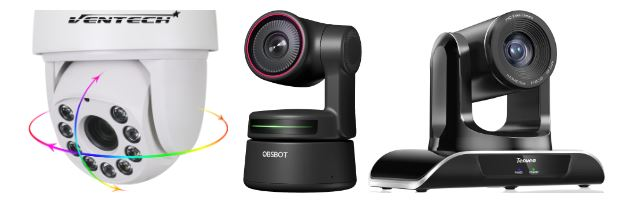
\includegraphics[scale=1]{Images/camera.jpg}\\
    \vspace{1.5cm}
    Philéas CURTIL, Thomas MAFILLE, Rémy MAILLARD \\
    \vspace{0.5cm}
    \vspace{1.5cm}
    \thedate \\
    \vspace{2cm}
    
\includegraphics[scale=0.7]{Images/Isep.jpg}\\
    \vspace{2cm}
    \small{\textit{Made with LaTeX}}

\end{titlepage}

\tableofcontents
\setlength{\parskip}{10pt}

\newpage

\section{Data visualization}

\begin{enumerate}[label={\color{blue}\arabic*)}]

    \item 
    When we load \textit{data-proj.mat}, we can see that there are two vectors in the file : 
    \begin{lstlisting}[style=Matlab-editor,language=Matlab]
    Name       Size       
    
    omega      1x20001            
    t          1x20001
  
    \end{lstlisting}
    
    \item 
    Plot of the angular speed \(omega\) as a function of time.
    
    \begin{multicols}{2}
    
        \begin{flushleft}
            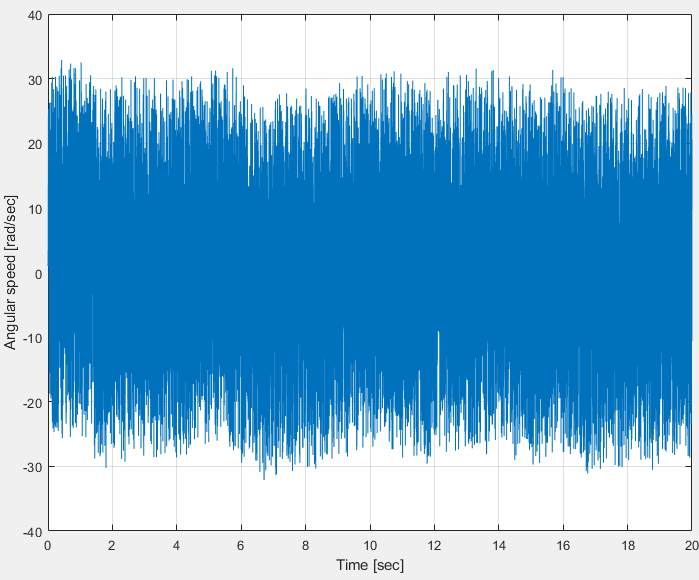
\includegraphics[scale=0.35]{Images/Figure 1.png}
            \captionof{figure}{Angular speed as a function of time}
            \label{Figure1}
        \end{flushleft}
        
    \columnbreak
    
    To obtain this graph :
    
    \begin{lstlisting}[style=Matlab-editor,language=Matlab, basicstyle=\small\ttfamily]
figure(1)
plot(t, omega)
grid on
hold on
xlabel('Time [sec]')
ylabel('Angular speed [rad/sec]')
        \end{lstlisting}
        
    \end{multicols}
    
    It is not possible to use the signal as it is now, mostly because there is too much information (too noisy) or the window is too large. This signal is continuous (analog). Electronic control devices requires digital signals.
    
\end{enumerate}

\newpage
\section{Analog filtering}

\begin{enumerate}[label={\color{blue}\arabic*)}]
    \setcounter{enumi}{2}
    \item The sampling period \(T_{e_1}\) can be calculated with :
    
        \begin{lstlisting}[style=Matlab-editor,language=Matlab, basicstyle=\small\ttfamily]
            Te1=t(2)-t(1)
    
            >>Te1 =
    
            1.0000e-03
      
        \end{lstlisting}

    \item
    Plot of the amplitude spectrum of \(omega(t)\), with the use of the workshop 5 :

    \begin{multicols}{2}
    
        \begin{flushleft}
            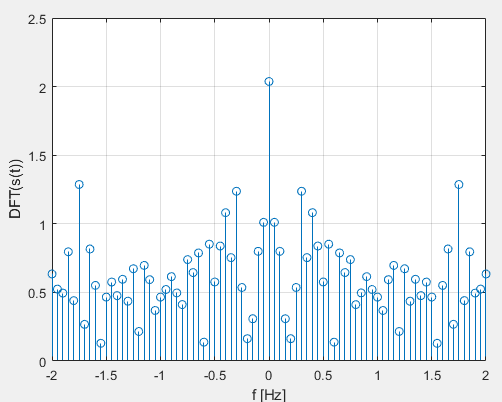
\includegraphics[scale=0.35]{Images/DFT.png}
            \captionof{figure}{DFT plot of \(omega(t)\)}
            \label{Figure2}
        \end{flushleft}
        
    \columnbreak
    
    To obtain this graph :
    
    \begin{lstlisting}[style=Matlab-editor,language=Matlab, basicstyle=\small\ttfamily]
% Plot of the DFT of omega(t)
Te2= 0.05; 
Fe2=1/Te2;
Tf=t(end);
N=Tf/Te2 ;

f1=-Fe2*(N/2-1)/N:Fe2/N:0;
f2=Fe2/N:Fe2/N:(N/2)*Fe2/N;
f = [f2,f1];
S= zeros(N,1);
for m=1:N
  for k=1:N
    S(m)=S(m)+omega(k)*exp(-1i*2*pi*m*k/N);
  
  end
end

figure(2)
stem(f,abs(S)/N)
grid on
hold on
xlim([-2 2])
xlabel('f [Hz]')
ylabel('DFT(\omega (t))')
        \end{lstlisting}
        
    \end{multicols}

    \item 
    The frequencies contained inside the signal are ranging from -2 Hz to 2 Hz with a step of 0.05.
    
    \(F_{max} = 2 Hz\)
    \newpage

    \item 
    The cutoff frequency is \(f_c = 2 Hz\). \\
    On Matlab :
    \begin{multicols}{2}
    
        \begin{flushleft}
            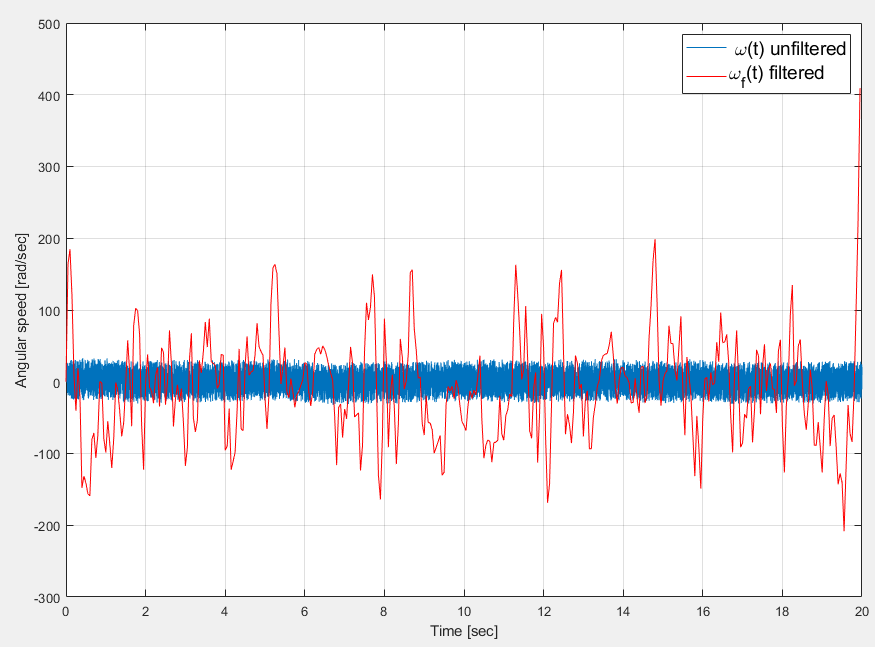
\includegraphics[scale=0.32]{Images/Omega_Filtered.png}
            \captionof{figure}{\(omega(t)\) filtered and unfiltered (\(omega_f(t)\))}
            \label{Figure3}
        \end{flushleft}
        
    \columnbreak

    To obtain this graph :
    
    \begin{lstlisting}[style=Matlab-editor,language=Matlab, basicstyle=\small\ttfamily]
% filter design
t1=0:Te2:t(end)-Te2;
fc1=2;
H1=tf(1,[1/(2*pi*fc1)  1]);
Sf=lsim(H1,S,t1);

% plot of filtered signal
figure(1);
plot(t1,Sf,'r')
grid on
legend(' \omega(t) unfiltered','\omega_{f}(t) filtered','Fontsize',14)
        \end{lstlisting}
        
    \end{multicols}

    On Simulink : 
    \begin{center}
        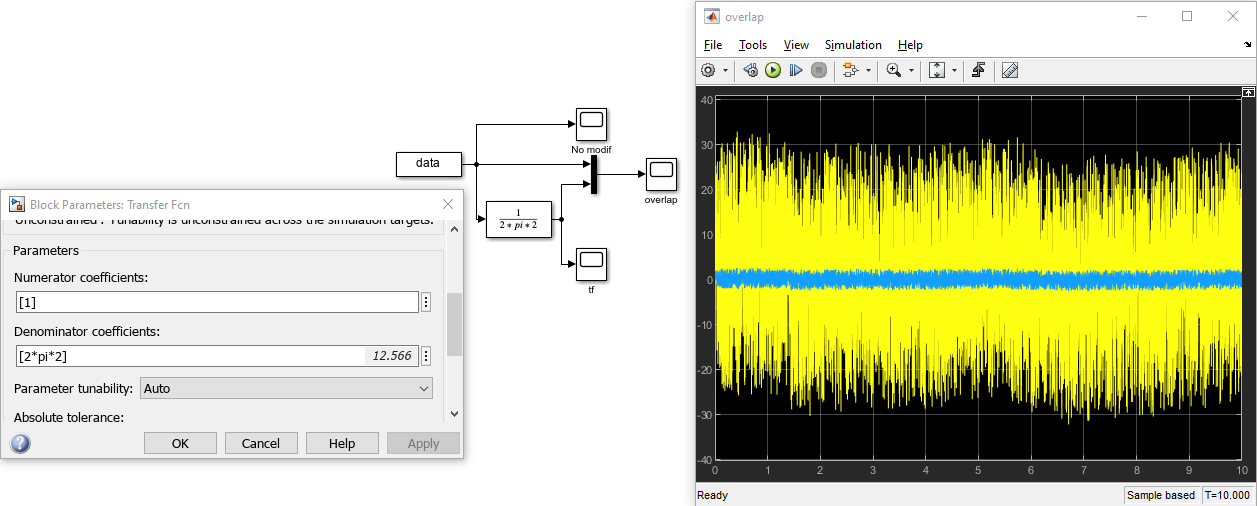
\includegraphics[scale=0.70]{Images/Simulink.png}
        \captionof{figure}{Simulink}
        \label{Figure4}
    \end{center}


    We need to add a part in the Matlab code as well :
    
    \begin{lstlisting}[style=Matlab-editor,language=Matlab, basicstyle=\small\ttfamily]
t_temp = t';
omega = omega';
data = [t_temp,omega];
        \end{lstlisting}
    \newpage
    \item
    Plot of the amplitude spectrum of \(omega_f(t)\), with the use of the workshop 5 :
    \begin{multicols}{2}
    
        \begin{flushleft}
            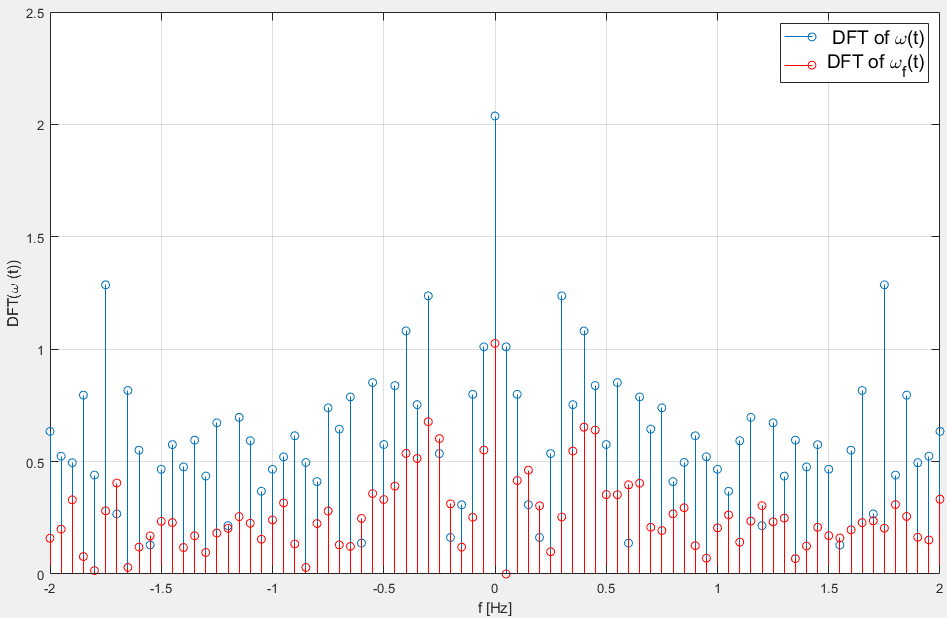
\includegraphics[scale=0.22]{Images/DFT_omega_f.png}
            \captionof{figure}{DFT plot of \(omega(t)\) and \(omega_f(t)\)}
            \label{Figure5}
        \end{flushleft}
    \columnbreak

    To obtain this graph :
    
    \begin{lstlisting}[style=Matlab-editor,language=Matlab, basicstyle=\small\ttfamily]
figure(2)
stem(f,abs(Sf)/N, 'r')
grid on
xlim([-2 2])
legend(' DFT of \omega(t)','DFT of \omega_{f}(t)','Fontsize',14)
        \end{lstlisting}
        
    \end{multicols}
    
\end{enumerate}

\newpage
\section{Sampling}

\begin{enumerate}[label={\color{blue}\arabic*)}]
    \setcounter{enumi}{7}

    \item 
    To create a vector \(omega_e(t)\) which contains the values of the vector \(omega_f(t)\) with a period between the values of \(T_{e2}\) = 0.05 sec.
    \begin{lstlisting}[style=Matlab-editor,language=Matlab, basicstyle=\small\ttfamily]
temp1 = 1:round(Te2/Te1):length(wf);
we=wf(temp1);
        \end{lstlisting}
    
    \item 
    To get the size of \(omega_e(t)\), we use :
    \begin{lstlisting}[style=Matlab-editor,language=Matlab, basicstyle=\small\ttfamily]
size(we)
        \end{lstlisting}
    \begin{flushleft}
            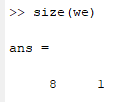
\includegraphics[width=0.25\linewidth]{Images/size_we.png}
            \captionof{figure}{Size of \(omega_e\)}
            \label{Figure5}
        \end{flushleft}

    \item 
    The new vector \(t_e\) which corresponds to the vector \(omega_e(t)\) can be created using :
    \begin{lstlisting}[style=Matlab-editor,language=Matlab, basicstyle=\small\ttfamily]
Te = (0:length(we)-1) * Te2;
        \end{lstlisting}
    Where we is \(omega_e(t)\).
    \newline
    \newline
    And we get those values for \(t_e\) :
    \begin{lstlisting}[style=Matlab-editor,language=Matlab, basicstyle=\small\ttfamily]
Te =

         0    0.0500    0.1000    0.1500    0.2000    0.2500    0.3000    0.3500
        \end{lstlisting}
    
    \item 
    Plot of \(omega_f(t)\) and \(omega_e(t)\) : 
    \begin{multicols}{2}
        \begin{flushleft}
            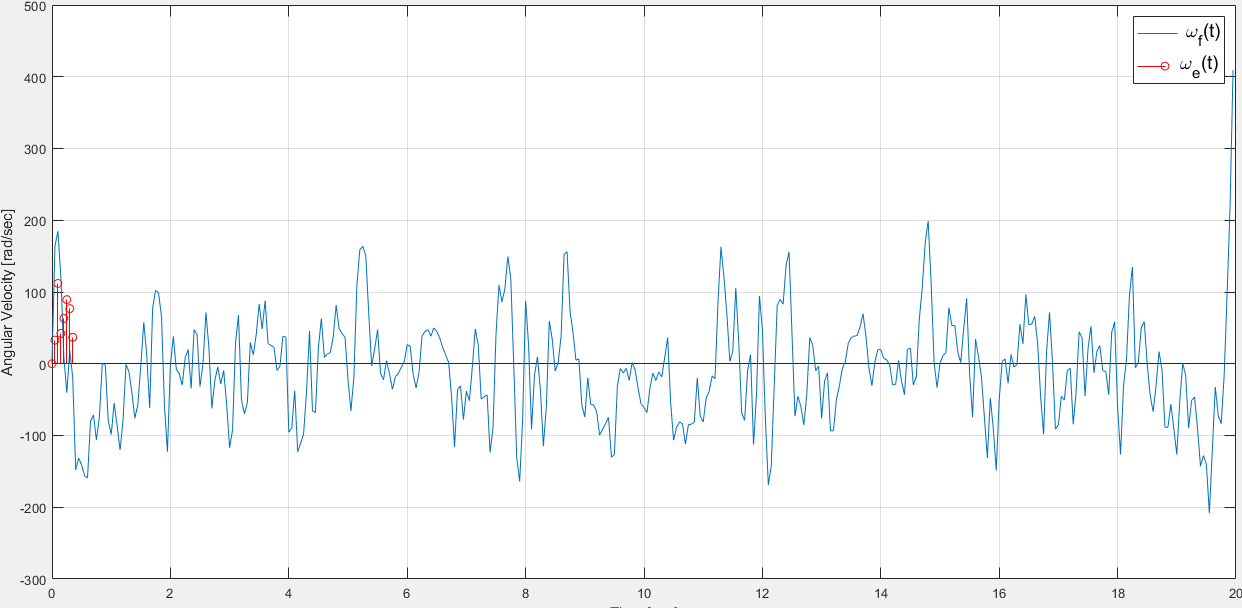
\includegraphics[width=0.75\linewidth]{Images/Wf_and_We.png}
            \captionof{figure}{Plot of \(omega_f(t)\) and \(omega_e(t)\)}
            \label{Figure6}
        \end{flushleft}

        \columnbreak

        \begin{lstlisting}[style=Matlab-editor,language=Matlab, basicstyle=\small\ttfamily]
figure(3)
plot(t1,wf)
xlim([10 12])
xlabel('Time [sec]')
ylabel('Angular Velocity [rad/sec]')
grid on
hold on
stem(Te,abs(we), 'r')
legend(' \omega_{f}(t)','\omega_{e}(t)','Fontsize',14)
        \end{lstlisting}
    \end{multicols}

    We can see that \(omega_e(t)\) is not visible because it is only display between 0 and 0.35 sec.
    \newpage
    
    \item 
    Plot of \(omega(t)\), \(omega_f(t)\) and \(omega_e(t)\) :
    \begin{multicols}{2}
        \begin{flushleft}
            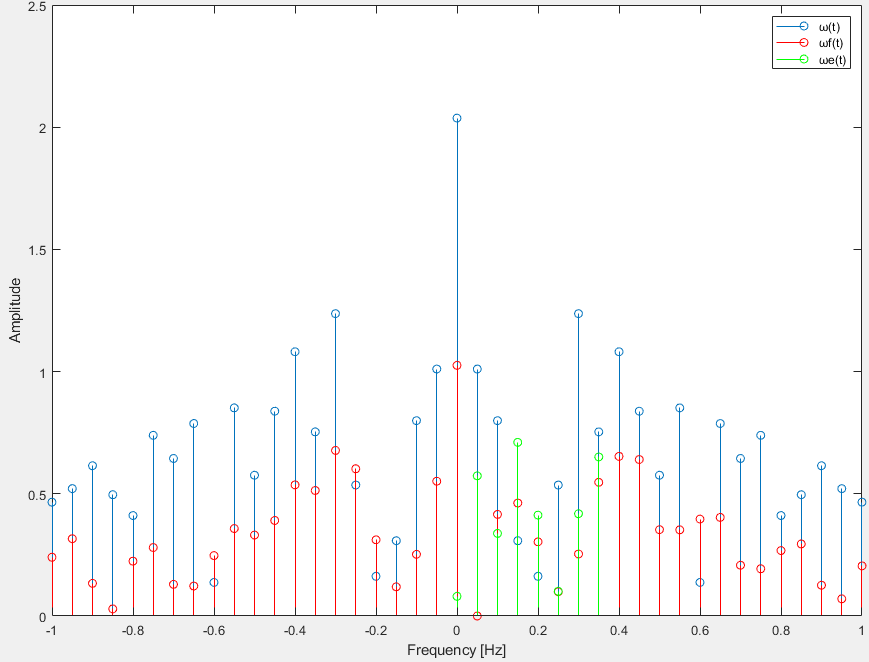
\includegraphics[width=1\linewidth]{Images/w_wf_weDFT.png}
            \captionof{figure}{Plot of \(omega_f(t)\) and \(omega_e(t)\)}
            \label{Figure6}
        \end{flushleft}

        \columnbreak

        \begin{lstlisting}[style=Matlab-editor,language=Matlab, basicstyle=\small\ttfamily]
we_dft = fft(we);

figure(4)
stem(f,abs(w)/N)
hold on
stem(f,abs(wf)/N, 'r')
stem(Te,abs(we_dft)/N, 'g')
xlabel('Frequency [Hz]')
ylabel('Amplitude')
legend('\omega(t)', '\omega_{f}(t)', '\omega_{e}(t)')
xlim([-1 1])
        \end{lstlisting}
    \end{multicols}

\end{enumerate}

\newpage
\section{Angular position and acceleration}

\begin{enumerate}[label={\color{blue}\arabic*)}]
    \setcounter{enumi}{12}

    \item 
    A
    
    \item 
    A

\end{enumerate}

\newpage
\section{Digital filtering}

\begin{enumerate}[label={\color{blue}\arabic*)}]
    \setcounter{enumi}{15}

    \item 
    A
    
    \item 
    A

\end{enumerate}

\end{document}